\chapter{QoS metrics}

If you go to the postal office to submit a packet, you will be offered different options.
In addition to the regular service, it is possible that an urgent service exists.
Probably there is also the possibility sending the packet as certified mail, and some option for delivery notification.
It is likely that there are also special services for packets that are voluminous or heavy.

QoS-enabled packet switched networks also offer different kinds of services for data packet delivery.
In this chapter, we will review the different metrics that are relevant for data networks.
This metrics can be used to establish \emph{service level agreements} (SLAs) which are contracts specifying the QoS expected from a network.
These contracts should also specify how the metrics are actually measured.

As an example, if a network guarantees a delay below 100 ms, it should be specified whether this makes reference to the maximum, the delay or the 95\% percentile.
The measures will also differ depending whether 5 minutes averages or 1 hour averages are considered.
This makes the specification of SLAs tricky.

\section{Delay}

Delay is the time that it is required to traverse the network from the entry point to the exit point.
Delay is normally considered for real-time services such as voice over IP (VoIP).
The total end-to-end delay is simply the sum of the delay suffered in each of the hops in the data network.
As an example, \ref{fig:four_hops} shows a network with four hops.

\begin{figure}[h]
\centering
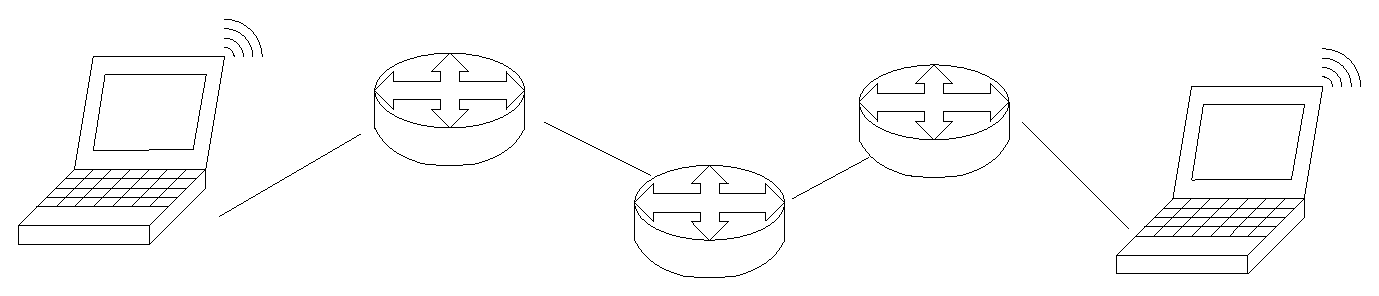
\includegraphics[width=\linewidth]{figures/four_hops.eps}
\caption{A network with two terminals, three routers and four hops.}
\label{fig:four_hops}
\end{figure}

In each hop, there are four different contributions to delay:
\begin{enumerate}
\item Processing: The time required for the router or switching device to put the packet on the outgoing interface queue.
Very short.
\item Queueing: Waiting time on the outgoing interface queue.
Very short if the queue is empty.
\item Transmission: The time required to put the packet on the transmission medium. It is a function of the packet length and transmission rate.
Short in high-speed transmission media.
\item Propagation: The time that it takes for the packet to travel the distance from the hop source to the hop destination.
Short time over short distances. 
And very long when it involves a trip to a geostationary satellite.
\end{enumerate}

\section{Jitter}
Jitter is the variation of delay.
This aspect is specially relevant for real-time and streaming applications.
These applications expect the packets to arrive regularly in time.
As an example, if the encoder application takes a voice stream and splits it into 20 ms chunks that are encoded and sent as packets, the receiver application will expect to receive one packet every 20 ms to reconstruct the voice stream.

If packets are sent every 20 ms but each of them requires a different time to traverse the network, the separation between packets will no longer be 20 ms at the receiving end.
Applications sensitive to jitter use a de-jittering buffer that holds some packets and feeds the decoder at regular intervals.
The packets that suffered a short delay in the network will wait for a longer time in the de-jitter buffer and the packets that suffered a longer delay in the network stay in the buffer for a shorter time.
With this technique, jitter is effectively suppressed at the expense of increasing delay.

\section{Round Trip Delay}

The round trip delay is the measure of delay used for elastic and interactive applications.
It is the time required for a packet from source to destination and then back to the source again.
You can easily find the round trip delay from your host using the ping command.

\begin{lstlisting}
$ ping www.happyforecast.com
PING happyforecast.com (184.107.100.65) 56(84) bytes of data.
64 bytes from s106.panelboxmanager.com (184.107.100.65): icmp_req=1 ttl=48 time=122 ms
64 bytes from s106.panelboxmanager.com (184.107.100.65): icmp_req=2 ttl=48 time=121 ms
64 bytes from s106.panelboxmanager.com (184.107.100.65): icmp_req=3 ttl=48 time=122 ms
64 bytes from s106.panelboxmanager.com (184.107.100.65): icmp_req=4 ttl=48 time=122 ms
64 bytes from s106.panelboxmanager.com (184.107.100.65): icmp_req=5 ttl=48 time=122 ms
64 bytes from s106.panelboxmanager.com (184.107.100.65): icmp_req=6 ttl=48 time=121 ms
^C
--- happyforecast.com ping statistics ---
6 packets transmitted, 6 received, 0% packet loss, time 5004ms
rtt min/avg/max/mdev = 121.864/122.066/122.181/0.230 ms
\end{lstlisting}

An interactive application (such as web browsing) requires a few round trip delays to complete the dialogue between the client and the server.
Furthermore, the round trip delay also limits how fast the TCP congestion window can grow.
The congestion window grows upon the reception of TCP acknowledgements.
If it takes long for the TCP acks to arrive, the congestion window grows slowly.

In fact, it becomes difficult to take fully advantage of connections with a high \mbox{bandwidth x delay} product.
These are known as ``long fat pipes'' or ``long fat networks'' (which is shortened as LFN and sometimes pronounced elephant), as explained in RFC 1072 \cite{rfc1072}.
